\section{Executable Representation and Mathematical Semantics}
\label{app:C}

\subsection{A world, its observations, and its evidence}
The executable interface summarizes a model output as
\begin{equation}
W=(\mathcal O,\mathcal G,\alpha,\mathcal R,\mathcal P).
\end{equation}
Here $\mathcal O$ contains typed physical instances, assemblies, parts, and interfaces. $\mathcal G$ assigns supported geometric primitives and frames. The observation binding $\alpha$ maps image observations to declared instances. $\mathcal R$ contains typed declarations, including hosts, floors, and connections. $\mathcal P$ records sources, active status, and explicit evidence links. These fields organize an inspectable output; they do not define a learned representation or recover missing image evidence automatically.

The JSON contract also permits semantic types and depictions. A repeated window type code is therefore different from a physical window instance. The operational \code{identity\_assignment} reader compares the instance IDs assigned to two singleton observations. Equal IDs return true and unequal IDs return false for this \emph{assignment} measurement. The reference comparison determines whether that assignment is correct. This operation does not prove physical identity from pixels. The separate physical-identity predicates require compatible physical referents, and different IDs alone do not prove that two physical objects differ.

The same distinction applies to ownership. \code{owner} is descriptive text; \code{owner\_id} is an explicit identity field. The evaluator does not derive household identity from a room's position or from a descriptive string. Ownership, geometric connection, and permission to traverse remain separate. A source ID identifies evidence in the output ledger; its presence does not establish that the source supports the claim.

\subsection{Coordinates, units, and supported transformations}
World coordinates use two horizontal axes and an upward $z$ axis. Each executable box has finite bounds $a_j<b_j$ in all three dimensions. A local frame acts through
\begin{equation}
\begin{bmatrix}x'\\1\end{bmatrix}
=\begin{bmatrix}P&t\\0&1\end{bmatrix}
\begin{bmatrix}x\\1\end{bmatrix},
\qquad P\in\{0,\!\pm1\}^{3\times3},\quad P^\top P=I,
\end{equation}
with exactly one nonzero entry in each row and column of $P$. Thus the implemented transforms are signed axis permutations and translations. The compiler transforms all eight corners of a box. It does not silently approximate an arbitrary rotated solid with its bounding box. Straight stairs must remain compatible with the supported horizontal-run and upward-rise convention after transformation.

The evaluator accepts declared normalized, meter, foot, and inch units. Normalized coordinates do not establish metric dimensions. For recognized metric units, numerical tolerance is
\begin{equation}
\epsilon_u=10^{-6}/c_u,
\end{equation}
where $c_u$ is meters per declared unit. For normalized or unrecognized units, it is $10^{-6}$ in the declared coordinate unit. \code{apply\_evaluation\_policy} replaces a model-supplied arithmetic tolerance with this fixed policy and preserves the original declaration for audit. Adding a distant object therefore does not change local tolerance. This tolerance controls numerical comparisons, not a permitted construction error or a human clearance standard.

\subsection{Material, free regions, and openings}
The primitives are \code{box}, \code{box\_union}, \code{stair\_run}, and \code{unknown}. A box union denotes its actual union, not its enclosing box. Rooms and corridors are spatial regions. Walls, slabs, obstacles, and tread bodies occupy material. Their spatial overlap with a room is not itself a collision between two solids.

For a material host $h$, let $B_h$ be the union of its input boxes and let $V_h$ contain its compatible, explicitly registered opening volumes. The compiler computes
\begin{equation}
M_h=B_h\setminus\bigcup_{o\in V_h}B_o.
\label{eq:material-difference}
\end{equation}
Both \code{subtract\_union} and \code{contains\_union} operate on component boxes. Subtraction partitions a box into at most six remaining boxes per cut; the implementation caps the resulting representation at 4,096 boxes. A colored opening drawn over a complete wall does not remove material unless the host registers that opening. Conversely, the final wall interface can recognize an already cut host with an equivalent registered void (Appendix~\ref{app:D}).

The geometric predicates have different boundary conventions. \code{intersects} requires positive-volume material overlap above tolerance; mere touching does not satisfy it. \code{contains} checks that subtraction leaves no region. \code{projected\_crossing} checks nonempty overlap in a selected coordinate projection and may include boundary contact. It does not imply three-dimensional intersection. \code{above} and \code{below} require horizontal component overlap and vertical interval separation, rather than ordering entity centroids. Consequently, these names must be interpreted through their stated predicates, not through an informal drawing impression.

\subsection{Straight stairs and supported interfaces}
A straight run specifies lower endpoint $p_0$, upper endpoint $p_1$, width $w>0$, tread thickness $t>0$, and integer step count $2\le n\le128$. Exactly one horizontal coordinate changes. Let $r$ be that run coordinate, $a$ the constant transverse coordinate, and $\Delta z=z_1-z_0>0$. Writing each tread in $(r,a,z)$ coordinate order, for $i=0,\ldots,n-1$, define
\begin{align}
r_i&=r_0+(r_1-r_0)i/n,& z_i&=z_0+\Delta z(i+1)/n,\\
T_i&=[\min(r_i,r_{i+1}),\max(r_i,r_{i+1})]
\times[a-w/2,a+w/2]\times[z_i-t,z_i].
\end{align}
The compiler expands the run into $\bigcup_iT_i$. This geometry represents tread material, not a complete structural stair or an occupant swept volume.

Connection labels are obligations to check. \code{stair\_connection} tests the declared endpoint interfaces, landing hosts, endpoint heights, and supported floor-level connection to the named rooms. A room floor uses its exposed lower free-space boundary; a material landing uses its exposed top. The landing bridge must connect to a free room-floor component after subtracting material immediately above that level. Area overlap and positive-length edge contact can connect these floor charts; a corner-only contact cannot. Material ending at the floor can support the route without blocking it.

A compound stair declares finite straight runs and material landings. Its parent material must equal the union of the declared parts. The implemented assembly is a connected, nonbranching, acyclic chain with two external interfaces; nested or curved assemblies are outside this interface. The evaluator separately sweeps material over tread tops. A full-width occupied stripe extending above a tread is a definite obstruction. A side overlap without that condition can remain unresolved. The test does not establish body-height clearance or every possible walking trajectory.

\subsection{Door channels, window hosts, and route scope}
The final door reader evaluates connected opening components against retained wall material and the material-plus-void envelope. A through channel needs supported exterior ports on opposite wall faces and real material anchors. This rejects blind pockets and prevents a void extending beyond a wall from inventing a false wall-normal direction. A door must also reach the shared floor, have compatible opposite-side room incidence, and have its cut registered. A complete material blockage rejects the connection; a partial obstruction remains unresolved without a body profile. A window-host query verifies its typed wall, cut, boundary incidence, and declared room, without treating the window as a traversable door.

The derived route graph contains only interfaces whose connection checks return true. Graph reachability is therefore reachability through supported interfaces in the declared fragment. It does not prove that the whole building is navigable. Non-\code{ALL} permission scopes are not implemented, and \code{accessible} always returns \code{UNKNOWN}/\neval. Neither shared ownership nor a projected crossing adds a graph edge.

\subsection{Unknown geometry and alternative completions}
The broader scientific specification allows several worlds consistent with incomplete evidence. For active qualified evidence $E$, write
\begin{equation}
\mathcal S(E)=\{W:W\models E\},\qquad
q(E)=v\ \text{only if}\ \mathcal S(E)\ne\varnothing\ \text{and}\ \forall W\in\mathcal S(E),\ q(W)=v.
\end{equation}
This is an interpretation principle, not an implemented continuous-world enumeration algorithm. The current instrument reads one submitted world with bounded proof patterns. Explicit unknown geometry, absent required geometry, unresolved hosts, and unsupported operators remain unresolved. It does not choose a hidden favorable completion. Geometric parameters can be marked \code{EVIDENCE\_\allowbreak SUPPORTED}, \code{HYPOTHETICAL\_\allowbreak COMPLETION}, \code{MIXED}, or \code{UNKNOWN}; these declarations do not independently validate their evidence. Multiple different completions may pass the same qualified relational obligations.

\subsection{A complete runnable software example}
Listing~\ref{lst:stair-fixture} is a five-entity synthetic fixture, not a model prediction or a measured building. All dimensions are hypothetical. The two observation IDs deliberately bind to the same stair. The frozen 2.2.1 compiler accepts the complete listing. In a fresh replay, \code{stair\_connects} and \code{interface\_reachable} are true, \code{same\_floor(lo,hi)} is false, and \code{accessible} is unknown. These outputs demonstrate the distinction between a verified interface and human accessibility.

\begin{figure}[htbp]
\centering
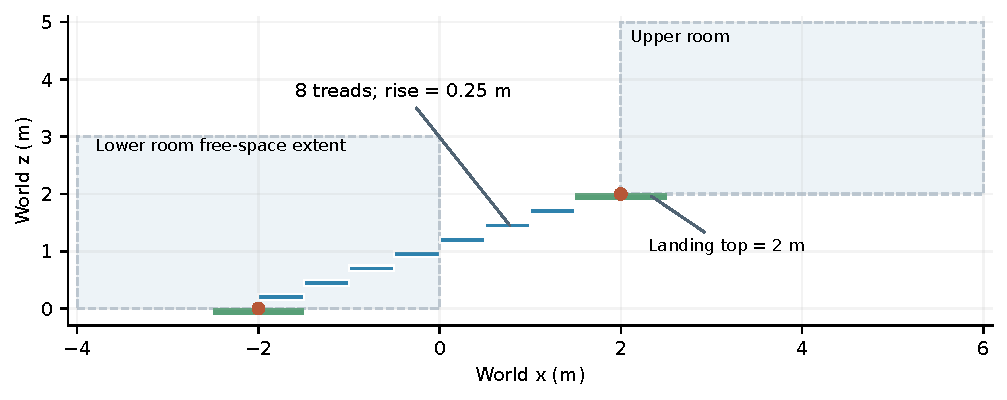
\includegraphics[width=.94\linewidth]{figures/verification/single_stair_fixture.pdf}
\caption{Compiled synthetic fixture in the $xz$ plane. Blue segments show the eight tread tops; green segments show material landings. Dashed boxes show room extents, not solid obstacles. The endpoint interfaces lie on the landing tops at $z=0$ and $z=2$ m. All plotted geometry comes from the same JSON listing.}
\label{fig:stair-fixture}
\end{figure}

\lstinputlisting[caption={Complete executable software fixture. Its observations are synthetic bookkeeping examples, with no image-grounding claim.},label={lst:stair-fixture},basicstyle=\ttfamily\fontsize{8}{9.5}\selectfont]{figures/verification/single_stair_listing.json}

The accompanying \sourcefile{figures/verification/verify_examples.py} checks this listing and four small door variants with byte-identical frozen code and Schema. The saved receipt contains five worlds and nine expected readouts. It is a software replay only; it adds no model trial or building sample.
